
% Created by tikzDevice version 0.5.3 on 2011-03-10 21:35:39
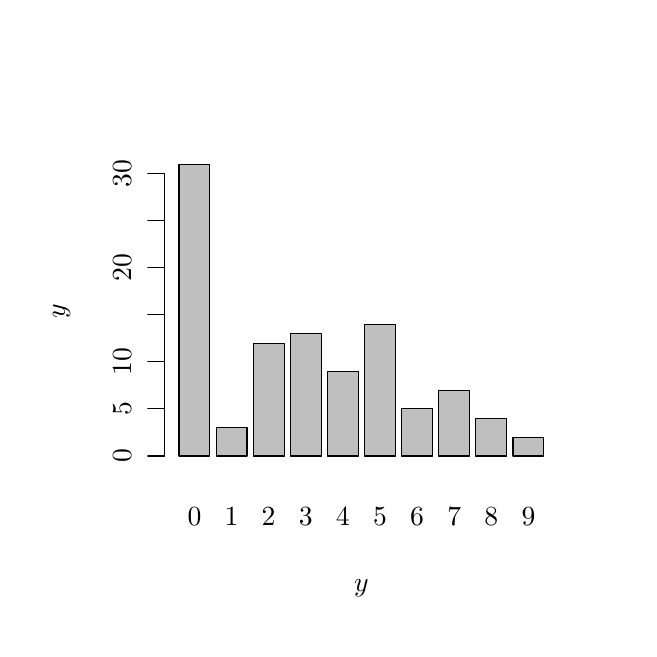
\begin{tikzpicture}[x=1pt,y=1pt]
\draw[color=white,opacity=0] (0,0) rectangle (216.81,216.81);
\begin{scope}
\path[clip] (  0.00,  0.00) rectangle (216.81,216.81);
\definecolor[named]{drawColor}{rgb}{0.50,0.23,0.81}
\definecolor[named]{drawColor}{rgb}{0.00,0.00,0.00}
\definecolor[named]{fillColor}{rgb}{0.75,0.75,0.75}

\draw[color=drawColor,line cap=round,line join=round,fill=fillColor,] ( 54.47, 62.25) rectangle ( 65.65,167.61);

\draw[color=drawColor,line cap=round,line join=round,fill=fillColor,] ( 67.88, 62.25) rectangle ( 79.06, 72.45);

\draw[color=drawColor,line cap=round,line join=round,fill=fillColor,] ( 81.29, 62.25) rectangle ( 92.47,103.04);

\draw[color=drawColor,line cap=round,line join=round,fill=fillColor,] ( 94.70, 62.25) rectangle (105.88,106.44);

\draw[color=drawColor,line cap=round,line join=round,fill=fillColor,] (108.11, 62.25) rectangle (119.29, 92.84);

\draw[color=drawColor,line cap=round,line join=round,fill=fillColor,] (121.52, 62.25) rectangle (132.70,109.83);

\draw[color=drawColor,line cap=round,line join=round,fill=fillColor,] (134.93, 62.25) rectangle (146.11, 79.25);

\draw[color=drawColor,line cap=round,line join=round,fill=fillColor,] (148.34, 62.25) rectangle (159.52, 86.04);

\draw[color=drawColor,line cap=round,line join=round,fill=fillColor,] (161.75, 62.25) rectangle (172.93, 75.85);

\draw[color=drawColor,line cap=round,line join=round,fill=fillColor,] (175.16, 62.25) rectangle (186.34, 69.05);
\end{scope}
\begin{scope}
\path[clip] (  0.00,  0.00) rectangle (216.81,216.81);
\definecolor[named]{drawColor}{rgb}{0.50,0.23,0.81}
\definecolor[named]{drawColor}{rgb}{0.00,0.00,0.00}

\node[color=drawColor,anchor=base,inner sep=0pt, outer sep=0pt, scale=  1.00] at ( 60.06, 37.20) {0%
};

\node[color=drawColor,anchor=base,inner sep=0pt, outer sep=0pt, scale=  1.00] at ( 73.47, 37.20) {1%
};

\node[color=drawColor,anchor=base,inner sep=0pt, outer sep=0pt, scale=  1.00] at ( 86.88, 37.20) {2%
};

\node[color=drawColor,anchor=base,inner sep=0pt, outer sep=0pt, scale=  1.00] at (100.29, 37.20) {3%
};

\node[color=drawColor,anchor=base,inner sep=0pt, outer sep=0pt, scale=  1.00] at (113.70, 37.20) {4%
};

\node[color=drawColor,anchor=base,inner sep=0pt, outer sep=0pt, scale=  1.00] at (127.11, 37.20) {5%
};

\node[color=drawColor,anchor=base,inner sep=0pt, outer sep=0pt, scale=  1.00] at (140.52, 37.20) {6%
};

\node[color=drawColor,anchor=base,inner sep=0pt, outer sep=0pt, scale=  1.00] at (153.93, 37.20) {7%
};

\node[color=drawColor,anchor=base,inner sep=0pt, outer sep=0pt, scale=  1.00] at (167.34, 37.20) {8%
};

\node[color=drawColor,anchor=base,inner sep=0pt, outer sep=0pt, scale=  1.00] at (180.75, 37.20) {9%
};
\end{scope}
\begin{scope}
\path[clip] (  0.00,  0.00) rectangle (216.81,216.81);
\definecolor[named]{drawColor}{rgb}{0.50,0.23,0.81}
\definecolor[named]{drawColor}{rgb}{0.00,0.00,0.00}

\node[color=drawColor,anchor=base,inner sep=0pt, outer sep=0pt, scale=  1.00] at (120.41, 13.20) {$y$
};

\node[rotate= 90.00,color=drawColor,anchor=base,inner sep=0pt, outer sep=0pt, scale=  1.00] at ( 13.20,114.41) {$\Prob{y}$
};
\end{scope}
\begin{scope}
\path[clip] (  0.00,  0.00) rectangle (216.81,216.81);
\definecolor[named]{drawColor}{rgb}{0.50,0.23,0.81}
\definecolor[named]{drawColor}{rgb}{0.00,0.00,0.00}

\draw[color=drawColor,line cap=round,line join=round,fill opacity=0.00,] ( 49.20, 62.25) -- ( 49.20,164.21);

\draw[color=drawColor,line cap=round,line join=round,fill opacity=0.00,] ( 49.20, 62.25) -- ( 43.20, 62.25);

\draw[color=drawColor,line cap=round,line join=round,fill opacity=0.00,] ( 49.20, 79.25) -- ( 43.20, 79.25);

\draw[color=drawColor,line cap=round,line join=round,fill opacity=0.00,] ( 49.20, 96.24) -- ( 43.20, 96.24);

\draw[color=drawColor,line cap=round,line join=round,fill opacity=0.00,] ( 49.20,113.23) -- ( 43.20,113.23);

\draw[color=drawColor,line cap=round,line join=round,fill opacity=0.00,] ( 49.20,130.23) -- ( 43.20,130.23);

\draw[color=drawColor,line cap=round,line join=round,fill opacity=0.00,] ( 49.20,147.22) -- ( 43.20,147.22);

\draw[color=drawColor,line cap=round,line join=round,fill opacity=0.00,] ( 49.20,164.21) -- ( 43.20,164.21);

\node[rotate= 90.00,color=drawColor,anchor=base,inner sep=0pt, outer sep=0pt, scale=  1.00] at ( 37.20, 62.25) {0%
};

\node[rotate= 90.00,color=drawColor,anchor=base,inner sep=0pt, outer sep=0pt, scale=  1.00] at ( 37.20, 79.25) {5%
};

\node[rotate= 90.00,color=drawColor,anchor=base,inner sep=0pt, outer sep=0pt, scale=  1.00] at ( 37.20, 96.24) {10%
};

\node[rotate= 90.00,color=drawColor,anchor=base,inner sep=0pt, outer sep=0pt, scale=  1.00] at ( 37.20,130.23) {20%
};

\node[rotate= 90.00,color=drawColor,anchor=base,inner sep=0pt, outer sep=0pt, scale=  1.00] at ( 37.20,164.21) {30%
};
\end{scope}
\end{tikzpicture}
